\section{RISC-V Compilation}

The final step of the project was to compile a simple RISC-V program and run it on the soft RISC-V processor on FPGA.
The program was written in C and compiled using the RISC-V GCC toolchain.
I had to create a startup file to initialize the stack pointer to the top of the memory module (2\,kB), but other than that, the program was straightforward.
I tried two different programs: a simple program that loops the RGB LED and toggles the LED cyclically, and a more complex program that uses the micros peripheral for doing faded PWM transitions in RGB cycling.
There is only the \texttt{main} function in both the programs and no other functions -- with a function call, the program would not work as intended.

The first program is shown below with the oscilloscope screen capture in Figure~\ref{fig:rgb_led_oscilloscope}.

\begin{minted}[fontsize=\small,linenos,frame=lines,framesep=2mm]{c}
#include "peripherals.h"

int main(void) {
volatile char *led = (volatile char *)LED_ADDR;
volatile char *rgb_r = (volatile char *)RGB_R_ADDR;
volatile char *rgb_g = (volatile char *)RGB_G_ADDR;
volatile char *rgb_b = (volatile char *)RGB_B_ADDR;

*rgb_r = 0xFF;
*rgb_g = 0xFF;
*rgb_b = 0xFF;

while (1) {
*led = 0xFF;
*rgb_b = 0xFF;
*rgb_r = 0x00;
int count = CLK_HZ >> 5;
for (volatile int i = 0; i < count; i++);
*led = 0x00;
count = CLK_HZ >> 5;
for (volatile int i = 0; i < count; i++);
*led = 0xFF;
*rgb_r = 0xFF;
*rgb_g = 0x00;
count = CLK_HZ >> 5;
for (volatile int i = 0; i < count; i++);
*led = 0x00;
*rgb_g = 0xFF;
*rgb_b = 0x00;
count = CLK_HZ >> 5;
for (volatile int i = 0; i < count; i++);
}
return 0;
}
\end{minted}

\begin{figure}[H]
    \centering
    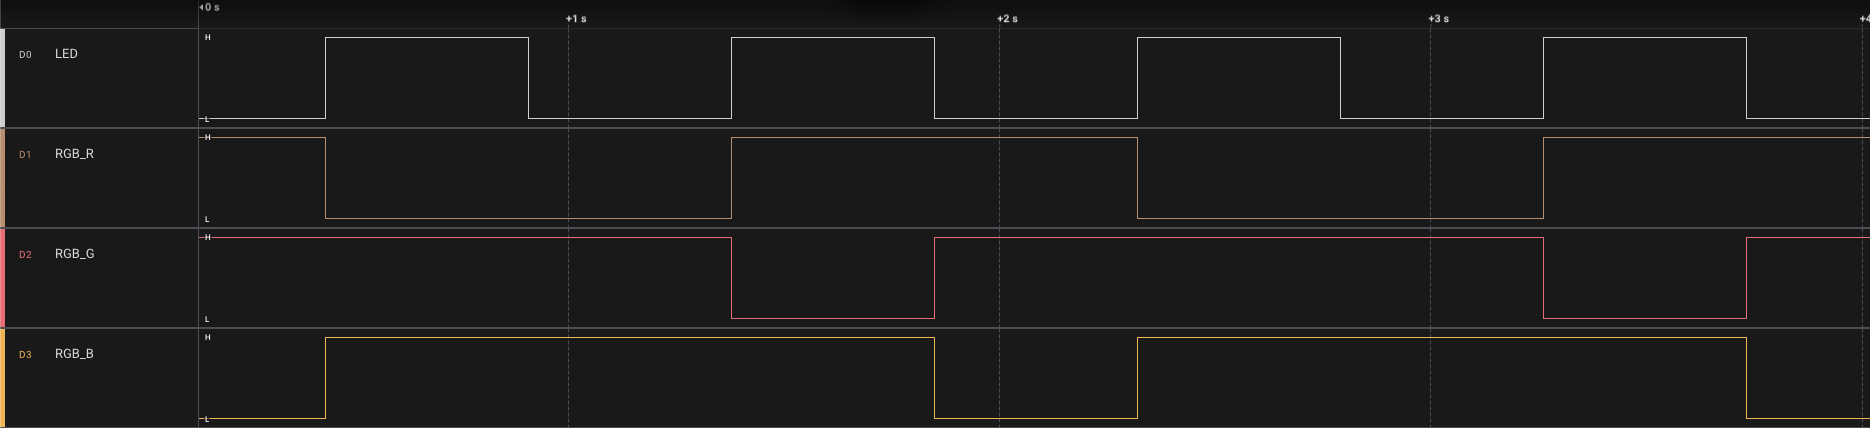
\includegraphics[width=\textwidth]{media/rgb_led_oscilloscope}
    \caption{Oscilloscope result for RGB LED and LED. The waveform shows the LEDs changing colors for a single loop. The LEDs were mapped to GPIO pins for debugging. The oscilloscipe has glitch filters enabled for 85\,ns to avoid the single-clock-period ($\sim$83\,ns) glitch when the PWM counter overflows for the sake of clarity.}
    \label{fig:rgb_led_oscilloscope}
\end{figure}